\documentclass[a4paper,titlepage,12pt]{scrartcl}
\usepackage[utf8x]{inputenc}
\usepackage[paper=a4paper,includefoot,includehead,left=30mm,right=20mm,top=20mm,bottom=20mm]{geometry}
\usepackage[T1]{fontenc}
\usepackage{graphicx}
\usepackage[ngerman]{babel}
%\usepackage
%[colorlinks=true,linkcolor=red,
% anchorcolor=black,citecolor=green,
% pagecolor=red,urlcolor=cyan,backref,]{hyperref}
\usepackage{cite}
\usepackage{url}
\usepackage[german]{varioref}
%Add a box around floats
\usepackage{float}
\floatstyle{boxed} 
\restylefloat{figure}

\setcounter{secnumdepth}{3}
\setcounter{tocdepth}{3}

\title{3D-Tumorvisualisation}
\subtitle{Seminararbeit}
\author{Uli Köhler}
%\institute[EMG]{Ernst-Mach-Gymnasium Haar}
\date{9.~November 2010}

\begin{document}
\maketitle\thispagestyle{empty}\newpage
\tableofcontents\thispagestyle{empty}\newpage
\section{Einleitung}\label{sec:introduction}
In dieser Arbeit sollen Methoden und Algorithmen dargestellt werden, die zur dreidimensionalen Visualisation von Tumoren in Echtzeit dienen. Hierzu werden zuerst in Kapitel \vref{ssec:requirements} die allgemeinen Anforderungen und in Kapitel \vref{ssec:applications}
Anwendungsmöglichkeiten für solche Systeme dargestellt. Darauf aufbauend werden in Kapitel \vref{ssec:concepts} die Konzepte und Algorithmen dargestellt, die im Rahmen dieser Arbeit entwickelt wurden. Zur anschaulichen Darstellung und als Beweis für die Implementierbarkeit dieser Konzepte in Software wurde begleitend zu dieser Arbeit ein Programm (`VERTEBRA`) geschrieben, anhand dessen in Kapitel \vref{ssec:implementations} Möglichkeiten der Implementation der zuvor dargestellten Konzepte und deren Anwendbarkeit in der modernen Medizin diskutiert werden. Da sich diese Arbeit auf dreidimensionale Visualisationssysteme beschränkt, werden in Kapitel \vref{ssec:3dnav} zusätzlich Verfahren zur Navigation im dreidimensionalen Koordinatensystem vorgestellt, wobei besonderen Wert auf die in Kapitel \ref{ssec:requirements} dargestellten Anforderungen gelegt wird.

Abschließend wird in Kapitel \vref{sec:augmentedreality} die Technik der `Augmented Reality` diskutiert, die in Zukunft eine wichtige Rolle in der medizinischen Visualisationstechnik und speziell im Bereich der Chirurgie spielen könnte. Zudem wird in diesem Kapitel die Anwendbarkeit der in dieser Arbeit vorgestellten Konzepte auf die Augmented Reality analysiert.

Aufgrund des geringen Umfangs dieser Arbeit von \pageref{appendixstart} Seiten wurden die folgenden Themen nicht im Detail behandelt.
\section{Echtzeit-Tumorvisualisationssysteme}\label{sec:vissystems}
\subsection{Anforderungen}\label{ssec:requirements}
\subsection{Anwendungsmöglichkeiten}\label{ssec:applications}
Schon heute werden verschiedene medizinische Visualisationssysteme in den verschiedensten Bereichen der Medizin eingesetzt. 
\section{Konzepte zur Visualisation von Tumoren}\label{ssec:concepts}
\begin{figure}[p]
\begin{center}
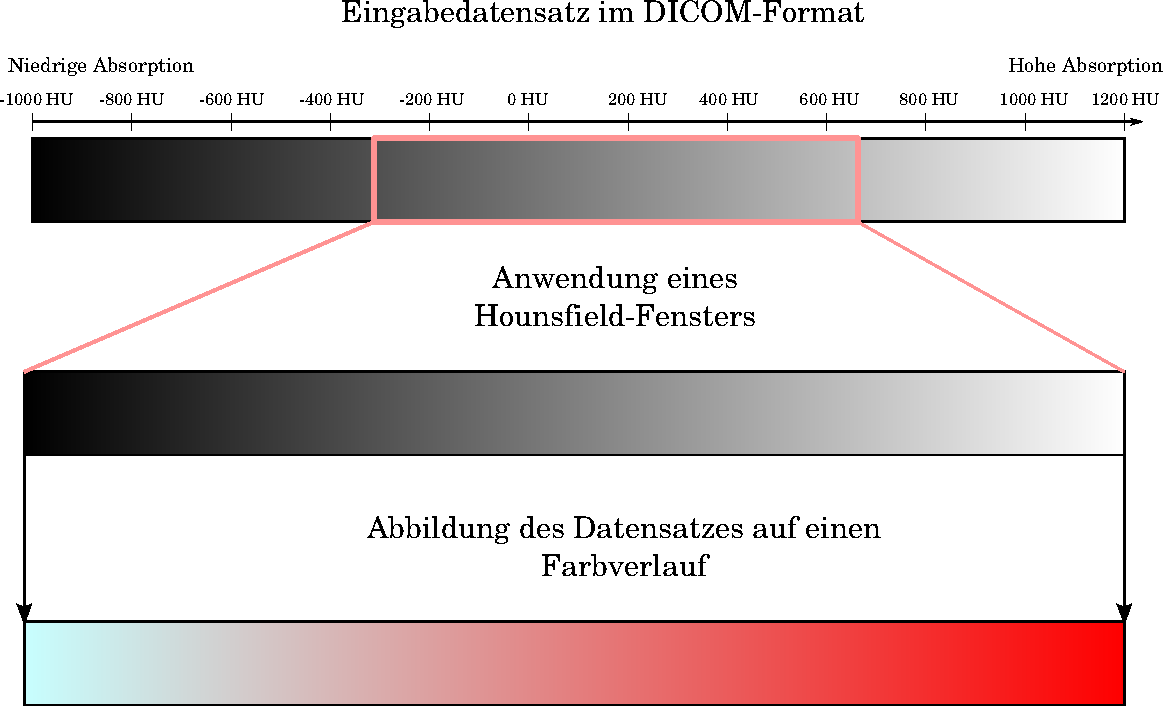
\includegraphics[width=\textwidth]{graphics/Tonemapping.pdf}
\caption{Verarbeitung von CT-Eingabedaten in VERTEBRA}
\label{gradientmapping-graphic}
\end{center}
\end{figure}
\subsection{Implementationsmöglichkeiten am Beispiel des Projektes VERTEBRA}\label{ssec:implementations}
Als Begleitprojekt zu dieser Arbeit wurde das Programm VERTEBRA (Volumetric Examiner for Radiological and Tomographical Experimental Basic Realtime Analysis) geschrieben, dessen Hauptzweck darin besteht, die Machbarkeit in dieser Arbeit vorgestellten Konzepte zu demonstrieren und im Rahmen der erreichbaren Genauigkeit vergleichbare Daten über die Echtzeittauglichkeit der Algorithmen und Verfahren zu liefern

VERTEBRA ist ein Proof-of-Concept-Projekt, zielt also nicht darauf ab, ein im medizinischen Alltag einsetzbares Produkt zu sein oder die für eine Zulassung nach dem Medizinproduktegesetz (bezogen auf deutsches Recht) notwendigen Vorraussetzungen zu schaffen.
\subsection{Grenzen der vorgestellten Konzepte}\label{ssec:limits}
\paragraph{Abhängigkeit von den Eingabedaten}
Die in dieser Arbeit vorgestellten Verfahren benutzen mathematische Verfahren, um eine Eingabedatenmenge variabler Größe in eine Menge an Eingabedaten zu übersetzen, die von spezialisierter Grafikhardware mathematisch in ein zweidimensionales Ausgangsbild umgerechnet wird, um auf einem visuellen Ausgabegerät, zum Beispiel einem Monitor angezeigt zu werden. Aufgrund dieser mathematischen Umrechnung basieren die Ausgabedatenmengen dieser Algorithmen ausschließlich auf den Eingabedatenmengen, die üblicherweise Datensätze aus tomografischen Scannern repräsentieren und den Konfigurationsparametern der Algorithmen.
\subsection{Methoden zur Berechnung von Visualisationsdaten}
\subsubsection{Vergleich von Software- und Hardwarealgorithmen}\label{ssec:swhwcomparison}

\subsubsection{Berechnung auf dem Hauptprozessor}\label{sssec:cpucalculation}
Die naheliegendste Möglichkeit, Operationen auf großen Mengen volumetrischen Daten durchzuführen, ist, die Berechnungen vom Hauptprozessor des Computers durchführen zu lassen. 
\subsubsection{Berechnung auf GPUs}\label{sssec:gpucalculation}
Da die Rechenleistung der Hauptprozessoren moderner Computer für viele der heutigen 3D-Anwendungen nicht mehr ausreicht, enthält ein Grossteil der heutigen Computer Grafikhardware, die in der Lage ist, 3D-Anwendungen zu beschleunigen. Hierbei berechnet der Hauptprozessor die darzustellenden Daten und gibt sie an die Grafikhardware weiter, die diese Daten mithilfe der GPU\footnote{GPU - Graphics Processing Unit - Grafikprozessor} in ein zweidimensionales Bild umwandelt (rendert), das beispielsweise auf einem Monitor angezeigt werden kann.

Um der GPU mitzuteilen, welche Objekte wo im dreidimensionalen Koordinatensystem auf welche Art gerendert werden sollen, müssen Programme ein Grafik-API\footnote{API - Application Programming Interface - Programmierschnittstelle} wie OpenGL oder DirectX benutzen. Im konkreten Fall von VERTEBRA fiel die Entscheidung aufgrund der Plattformunabhängigkeit und der Erfahrung der Autors in diesem Bereich.

Neuere GPUs können ausserdem so genannte Shader ausführen - kleine Programme, die für bestimmte Untereinheiten der zu visualisierenden Objekte ausgeführt werden. OpenGL stellt hierfür die Shaderprogrammiersprache GLSL\footnote{GLSL - [Open]Graphics Layer Shading Language - OpenGL-Shadersprache} zur Verfügung, die in \cite{Rost2006} für die OpenGL-Version 2.0 ausführlich beschrieben wird. Nach \cite[Seite 38-47]{Rost2006} können in dieser Sprachversion die folgenden Typen von Shadern unterschieden werden\footnote{Geometry-Shader sind im in \cite{Rost2006} benutzten Standard OpenGL 2.0 nicht enthalten und werden daher an dieser Stelle nicht aufgeführt}:
\begin{itemize}
 \item Vertex\footnote{Vertex - Ein einzelner Punkt im Raum - Vgl. \cite[Seite 664]{Wright2000} bzw. \cite[Seite 685]{Rost2006}}-Shader
 \item Fragment\footnote{Fragment - Datensatz bestehend aus der Information, die nötig ist, um ein Pixel zu zeichnen\\Vgl. \cite[Seite 675]{Rost2006}}-Shader
\end{itemize}
Die Shader-Prozessoren (Untereinheiten der GPU, die die Shader ausführen), arbeiten massiv parallel, führen also
\subsubsection{Berechnung auf FPGAs}
Abgesehen von den bereits diskutierten Möglichkeiten ist mit so genannten FPGAs\footnote{FPGA - Field Programmable Gate Array} eine weitere Form der Hardwarebeschleunigung für die medizinische Visualisationstechnik vorhanden. FPGAs sind ICs\footnote{IC - Integrated Circuit - Integrierter Schaltkreis}, bei denen nach der Herstellung eine anwendungsspezifische Programmierung und Konfiguration möglich ist (\cite{Kibritev2009}, Kapitel 1.7.1, Seite 16). Daher sind die Produktionskosten für ein auf FPGAs basierendes Visualisationssystem wesentlich geringer als bei dedizierter Hardware, die für eine bestimmte Aufgabe gefertigt wurde und nicht nachträglich programmierbar ist. Wie bereits in Kapitel \vref{ssec:swhwcomparison} diskutiert stellt Bruckner in \cite{Bruckner2008} Nachteile von hardwarebasiertem Rendering gegenüber softwarebasierten Darstellungen in Bezug auf große volumetrische Datensätze dar. FPGAs erlauben, wie Leeser et al. in \cite{Leeser2005} mithilfe einer Implementation des Parallel-Beam Backprojection-Algorithmus zeigen, eine performante Implementation dieser Softwarealgorithmen. In \cite{Thomas2009} findet sich ein Vergleich die Performanz von CPU-, GPU- und FPGA-basierten Systemen anhand von PRNGs\footnote{PRNG - Pseudo-random number generator - Pseudozufallszahlengenerator} - wie aus Tabelle 6 ersichlich liefert das im Experiment benutzt FPGA-basierte System bei zwei der drei dargestellen Verteilungen, die jeweils unterschiedliche Algorithmen benötigen bessere Resultate (also eine größere Zahl generierter Zufallszahlen pro Zeiteinheit) als die anderen getesteten Plattformen.
\subsubsection{Surface Rendering}
Die in dieser Arbeit behandelten Methoden beschränken sich auf das Volume Rendering (`Volumenrendern`), d.h. die Daten werden unter Beachtung der räumlichen Information gerendert. Als Alternative bietet sich das so genannte Surface Rendering (`Oberflächenrendern`) an, bei dem durch mathematische Verfahren Oberflächen im Datensatz gesucht werden, die dann als zusammenhängende Fläche gerendert werden. 

Kuszyk et al. stellen in \cite{Kuszyk1996} die Nachteile des Surface Renderings gegenüber dem Volume Rendering dar. Als Beispiel für einen Nachteil des Surface Rendering wird dargestellt, dass Läsionen unter Knochen verborgen werden während Volume Rendering-Algorithmen diese korrekt darstellen (Quelle: \cite{Kuszyk1996}, Abstract). Da die Publikation jedoch schon 1996 veröffentlicht wurde, gelten die Resultate unter Umständen für die heutigen Algorithmen und hochauflösenden Tomographen. Eine aktuellere Darstellung liefern Udupa et al. in \cite{Udupa2009}. Die Autoren kommen zu dem Schluss, dass Surface Rendering-Algorithmen im Bereich der Informationsdarstellung einen kleinen Vorteil gegenüber volumenbasierten Algorithmen haben und außerdem durch den geringeren Bedarf an Rechenzeit und Speicherplatz überlegen sind. Auch \cite{Bruckner2008} thematisiert den Vergleich von Oberflächen- und Volumenrendering, kommt aber im Gegensatz zur vorgenannten Publikation zum Schluss, dass der Mehraufwand an Rechenzeit und Speicher die Mehrinformation wert, die im gerenderten Bild angezeigt wird - tatsächlich würde beim Rendern der Oberflächen eine Dimension verloren gehen, da das Innere von Objekten verborgen bleibt (Quelle: \cite[Seite 6f.]{Bruckner2008}).

\section{Augmented Reality - Zukunft von Visualisationssystemen?}\label{sec:augmentedreality}
In den letzten Jahren wird neben den herkömmlichen Geräten zu Darstellung der Informationen medizinischer Informationssysteme (z.B. Bildschirme) intensiv an der so genannten `Augmented Reality` geforscht. Dieser Begriff, der sich mit 'Erweiterte Realität' (Quelle: \cite[Seite 1]{Toe2010}) übersetzen lässt, beschreibt laut \cite{Suthau2002DE} (Seite 1; Englische Publikation: \cite{Suthau2002}) das Konzept, reale Bilder mit zusätzlichen Informationen zu ergänzen.

\appendix \label{appendixstart}
\section{Anleitung zur Übersetzung von VERTEBRA}
Um den Quellcode von VERTEBRA in Maschinencode zu übersetzen, werden die folgenden Hilfsprogramme bzw. Bibliotheken benötigt:
\begin{itemize}
 \item C++-Compiler kompatibel zu ISO/IEC C++ 2003
 \item Qt Software Development Toolkit (SDK): minimal Version 4.7.0 = Qt SDK 2009.05.1
 \item DCMTK 3.5.4
\end{itemize}

Das Qt SDK kann von \url{http://qt.nokia.com} bezogen werden; die DCMTK-Bibliothek, die zum einlesen von DICOM-Daten benutzt wird, wird vom OFFIS e.v. (Oldenburger Forschungs- und Entwicklungsinstitut für Informatik, \url{http://offis.de}) auf \url{http://www.dcmtk.org/dcmtk.php.de} zu Verfügung gestellt.

Das Programm wurde mit der folgenden Konfiguration erfolgreich getestet (siehe auch Kapitel \vref{apdx:testplatform}):
\begin{itemize}
 \item C++-Compiler: GNU Compiler Collection \textit{gcc (Ubuntu/Linaro 4.4.4-14ubuntu5) 4.4.5}
 \item Qt SDK: 4.7.00 = Qt SDK 2009.05.1
\end{itemize}

\section{Testplattform}\label{apdx:testplatform}
Die in dieser Arbeit vorgestellten Geschwindigkeitsmessungen wurden auf der folgenden Plattform durchgeführt:
\begin{itemize}
  \item Dell Inspiron 530
  \item CPU: Intel\textsuperscript{\textregistered} Core\texttrademark 2 Duo E8300; 2.83GHz Taktfrequenz
  \item Betriebssystem: KUbuntu 10.10 x86\_64; Kernel 2.6.35-22-generic x86\_64
  \item Grafikhardware: NVidia\textsuperscript{\textregistered} GeForce 9400 GT, PCI Express x16\\
	Treiber 260.19.06 (Konfiguration: High Performance)
\end{itemize}
\section{Quellcode von VERTEBRA}
\section{Doxygen-Dokumentation von VERTEBRA}
\newpage
%\nocite{*}
\renewcommand\refname{Literatur- und Quellenverzeichnis}
\bibliographystyle{alphadin}
\bibliography{visualization}
\section{Selbstständigkeitserklärung}
Hiermit erkläre ich, dass ich die vorliegende Arbeit in allen Teilen selbstständig verfasst habe und keine anderen als die angegebenen Quellen und Hilfsmittel (einschließlich Onlinequellen und elektronischer Medien) benutzt habe.
\end{document}
